\section{Implementation}


% what's happening
% client-server architecture - structure - see figure

\begin{figure}
\centering{
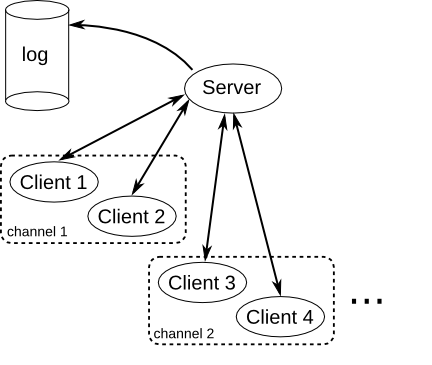
\includegraphics[width=0.6\columnwidth]{client-server.png}
}
\caption{Structure of the server-client
  relationship.}
\label{fig:server-client}
\end{figure}

The game is implemented using a client-server architecture illustrated
in Figure \ref{fig:server-client}. The client-server interaction is as
follows:

\begin{enumerate}
\item A player requests the game's webpage. The http server sends all game files.
\item The game's client-server connection is established.
\item The server assigns the client either to a channel containing
  only one player or a new channel.
\item Once two clients are in a channel, the server sends the signal to start
  to the clients.
\item The server listens and passes on any messages sent between
  players.
\item The server logs all movements in the game world and the
  communication between the two players.
\end{enumerate}


% how implemented; technology used

Since we would like to use this game to collect human-human
conversations and evaluate dialog systems over the Internet, it should
be as easy as possible to run the client. Therefore, we decided to
develop a browser based-game. Both the client and the server are
written in JavaScript.

% crafty.js - rendering/drawing to screen, collision detection, event management
The client uses Crafty\footnote{http://craftyjs.com}, a JavaScript and
HTML5 game engine, which facilitates drawing the game area into the
browser window, event management and collision detection. In the
beginning of the project, we explored a number of JavaScript game
engines and settled on Crafty because it seemed to satisfy our needs,
was under active development and came with many tutorials and good
documentation.


% node.js + express - to run server written in javascript,

The server is built on Node.js\footnote{http://nodejs.org/}, a
server-side JavaScript framework. In particular, the express
module\footnote{http://expressjs.com/} is used to create an HTTP
server, and the in-game client-server communication is implemented
using Socket.IO\footnote{http://socket.io}.

% socket.io - connect the clients to server

%% The game was created in javascript using the Crafty JS game engine
%% \cite{craftyJS}. Crafty JS provided an intuitive, understandable
%% environment to develop game and was cross compatible with all modern
%% browsers. However, the main motivation for using Crafty JS was the
%% abundance of tutorials and the well-structured documentation of the
%% game engine. This greatly reduced the time needed to learn how to use
%% the game engine which allowed more time for development.  The main
%% parts of Crafty JS used were the collision detection components and
%% the components used to draw objects to the screen. Both helped to
%% simplify the process of creating the game.  Node JS was used to create
%% the networking for the game \cite{nodeJS}. More specifically, the
%% server utilized the express and socket IO modules that each run using
%% node JS. Each module is responsible for a different part of the
%% communication between the server and the client. The general structure
%% of the communication between the server and the client is outlined by
%% the pseudocode in Figure \ref{fig:server-client}.


%% As detailed by the figure, the first part of the interaction between
%% the server and the client is initiated when a client logs onto the
%% specific website. When a connection occurs, the server sends all files
%% necessary to play the game to the client.  These files include the
%% javascript files, any image files that the game uses, and an index
%% html file. This is accomplished through the use of the express module
%% \cite{express}. The express module allowed for the simple setup of an
%% HTTP server that listened for any clients connecting to the website.

%% After the files have been received, the client begins to run the
%% game. The first thing that happens in the game is that it establishes
%% a connection with the server using Socket IO \cite{socketIO}. The
%% purpose of Socket IO is to create an easy method of transmitting data
%% between the client and the server and vice versa. Also, since the game
%% is played in groups of two players, the server needed to be able to
%% have different channels for players to play on. Socket IO could
%% provide this using a built-in component called a room that had the
%% same behavior as channels. This made step three of the server-client
%% relationship trivial and therefore allowed me to spend more time on
%% other aspects of the game instead of creating channels from scratch.

%% The last two steps of the server client relationship as shown in
%% figure three are handled using Socket IO. Socket IO transmits
%% information between the server and the client through a process of
%% listening for and emitting different events. Each event that is
%% emitted by either the client or the server has data attached to it
%% that is received by whatever is listening for that event. For example,
%% in step four when the server sends data to the player to start the
%% game it does this by emitting a “setup” event with the data
%% attached. The client side is listening for this “setup” event and when
%% it hears this event, it also gets the attached data. As described in
%% step five, there are many different events that are emitted throughout
%% the course of the game that are all handled in this same manner using
%% Socket IO.
